\chapter{Entrelazamiento}
\label{ch2_entrelazamiento}


%CAMBIAR ESTO PARA PERSONALIZARLO A MI GUSTO
\pagestyle{fancy}
\fancyhf{}
\fancyhead[LE]{\nouppercase{\rightmark\hfill}}
\fancyhead[RO]{\nouppercase{\leftmark\hfill}}
\fancyfoot[LE,RO]{\hfill\thepage\hfill}

Entrelazamiento en mecánica cuántica. El entrelazamiento, también conocido como acción espeluznante a la distancia, es un recurso importante en la mecánica cuántica. Este fenómeno no tiene un correlato clásico, ya que lleva a fenómenos que son inexplicables mediante la teórica no cuántica de la física, pero tiene cierta analogía con las correlaciones que se encuentran en la física clásica. El ejemplo mas común de esta analogía es el caso de una masa extensa clásica que está en reposo, y espontáneamente explota mediante procesos internos en dos partes. Imaginemos que esta explosión genera cierto momento angular sobre cada una de las partes. Por conservación del momento angular, que inicialmente es cero, también así lo debe ser luego de la explosión, por lo tanto, si yo me encuentro con uno de estos pedazos de la masa extensa, y le mido su momento angular, se con certeza que el momento angular de la otra masa debe ser exactamente el mismo, pero con signo opuesto para que la suma de momentos angulares sea nula. Lo mismo sucederá con el impulso. Estas cantidades físicas están perfectamente anticorrelacionadas entre si. El entrelazamiento es un fenómeno similar, pero que ciertamente no es el mismo. El entrelazamiento es un fenómeno que es no local. Esto desconcertó a mucha gente, y lo sigue haciendo, pero los experimentos no mienten, y esta es una realidad que tenemos que aceptar. Para dar con esta conclusión y corroborar experimentalmente que el entrelazamiento es un fenómeno no local, hay que mirar el espectacular trabajo de John Bell, físico irlandés de natalidad, al que se le ocurrió un experimento el cual podría ser medido, cuyo resultado daría resultados diferentes dependiendo de si uno acepta o no acepta la no localidad del entrelazamiento. Este experimento fue realizado y se corroboro que efectivamente, la realidad debe ser cuántica y el entrelazamiento es un fenómeno no local. Estas son conocidas como las desigualdades de Bell. 

La verdad que no se para que escribí todo esto pero bueno, lo dejo por acá. Ahora vamos a mirar medidas de entrelazamiento. En particular, estas son sacadas del review de Horodceki$^n$ \cite{quantumentanglementhorodecki}. En la seccion XV.B discuten diferentes medidas de entrelazamiento bipartito, algunas de las cuales se pueden generalizar a estados multipartitos. Cambien, interesantemente, dan una receta para convertir medidas de entrelazamiento para estados puros, generalizandolas para estados mixtos mediante una suma convexa. Sin mas, comencemos.
\section{Medidas de entrelazamiento basadas en distancia}
Esta clase de medidas de entrelazamiento están basadas en la intuición de que un estado separable no esta entrelazado, y si nosotros tenemos una medida de distancia en el espacio de estados, entonces un estado que es muy parecido y por lo tanto esta muy cerca de un estado separable, será poco entrelazado, aumentando esto mientras mas se aleje el estado de algun estado separable. Formalmente podemos decir, dada una medida de distancia $\mathcal{D}$ entre estados en un espacio de estados $\mathcal{S}$, entonces
\begin{equation}
    E_{\mathcal{D},\mathcal{S}}(\rho)=\inf_{\sigma\in\mathcal{S}}\mathcal{D}(\rho,\sigma)
\end{equation}
donde particularmente tenemos que decir quienes son $\sigma\in\mathcal{S}$. El conjunto $\mathcal{S}$ es el conjunto que es cerrado ante operaciones LOCC. Originalmente se consideraba $\mathcal{S}$ como el estado de estados separables. Pero esto no es necesario, o no es algo cierto si se quiere. Esta distnicion surge de que para sistemas de muchas particulas, hay diferentes clases de entrelazamiento, las cuales surgen de clasificar estados segun si podemos transformar un estado en otro mediante LOCC. Es decir, si usando solo LOCC podemos ir de un estado a otro, entonces estos pertenecen a una misma clase. Esta clasificacion hace que haya diferentes tipos de entrelazamiento al aumentar la cantidad de subsistemas, por ejemplo, para un sistema tripartito $\mathcal{H}=\mathcal{H}_1\otimes\mathcal{H}_2\otimes\mathcal{H}_3$. Acá hay algunas tecnicidades sobre la definición de la distancia $\mathcal{D}$, pero no nos vamos a meter en eso. Solo hay que saber que esta tiene que ser no-negativa y que esto implica que la medida de entrelazamiento tiene que ser monotona. La monotonicidad de la medida nos asegura que el entrelazamiento no crece ante LOCC, lo cual es una propiedad necesaria para una medida fiel de entrelazamiento, ya que si operamos con LOCC sobre un estado, siempre deberiamos quedar en la misma clase de entrelazamiento y no deberia aumentar. En \cite{verdalplenio1998} se encontraron dos medidas que satisfacen estas condiciones y ademas son convexas, estas son la métrica de Bures $B^2=2-2\sqrt{F(\rho,\sigma)}$ donde $F(\rho,\sigma)=[\text{Tr}(\sqrt{\rho}\sigma\sqrt{\rho})^{1/2}]^2$ es la fidelidad, y la segunda medida es la entropía relativa $S(\rho|\sigma)=\text{Tr}\rho(\log\rho-\log\sigma)$. Entonces podemos decir que 
\begin{equation}
     E_{\mathcal{D},\mathcal{S}}(\rho)=\inf_{\sigma\in\text{SEP}}\text{Tr}\rho(\log\rho-\log\sigma)
\end{equation}
es la \textit{entropía relativa de entrelazamiento}, que nos sirve como una medida de entrelazamiento, y es una medida fundamental ya que la entropía relativa es una de las funciones mas importantes en la teoría de la información cuántica. Hay otras versiones que calculan la distancia con respecto a los estados PPT \cite{Rains2000} y a los estados nondistillable \cite{Vedral1998}.

Ahora pasamos a ver como generalizar algunas medidas de estados bipartitos a estados multipartitos para estados puros, y luego tenemos que realizar una suma convexa para generalizar a estados mixtos. 

Existen algunas funciones que son sumas de medidas de entrelazamiento bipartito. Por ejemplo \textbf{global entanglement} \cite{MeyerWallach2001} que es la suma de las concurrencias de cada qubit vs los demás, entre otras medidas que son similares. Estas medidas no son una medida real de entrelazamiento multipartito, ya que no consideran entrelazamiento entre k-partes. La primera medida no obvia es el 3-tangle \cite{Coffman2000} 
\begin{equation}
    \tau(A:B:C)=\tau(A:BC)-\tau(AB)-\tau(AC)
\end{equation}
donde los $\tau$s del lado derecho son los 2-tangle, que son el cuadrado de la concurrence. El problema de esta medida es que puede ser 0 para algunos estados que presentan entrelazamiento entre las 3 partes, como los estados W. Por suerte no son cero para los estados GHZ. Aca vemos que el entrelazamiento tripartito tiene dos clases diferentes de estados entrelazados, que en esta medida, uno se pierde de la mitad de los estados. Hay intentos de generalizar esto. En \cite{Lohmayer2006} se computo un convex roof para el 3-tangle para una mezcla de estados GHZ y W. Luego del tangle, se introdujo un concepto para medir en sistemas tripartitos que salio del contexto de asymptotic rate of transitions \cite{Linden1999a}:
\begin{equation}
    E(\psi)=E_R(\rho_{AB})+S(\rho_C)
\end{equation}
donde $\rho_{AB,C}$ son reducciones de $\psi_{ABC}$.

El problema de estas medidas presentadas, es que siempre nos perdemos de alguna propiedad de entrelazamiento, no hay ninguna medida genuina de entrelazamiento tripartito. Busque un poco en internet y encontré un paper de unos chinos \cite{} \text{https://www.polyu.edu.hk/ama/profile/gfzhang/Research/GLW+\_PRA24.pdf} que encuentran una manera genuina de usar alguna medida de entrelazamiento bipartito para obtener una medida de entrelazamiento tripartito. Esta idea se basa en medir el área de un triangulo que representa los entrelazamientos bipartitos del sistema:
\begin{figure}
    \centering
    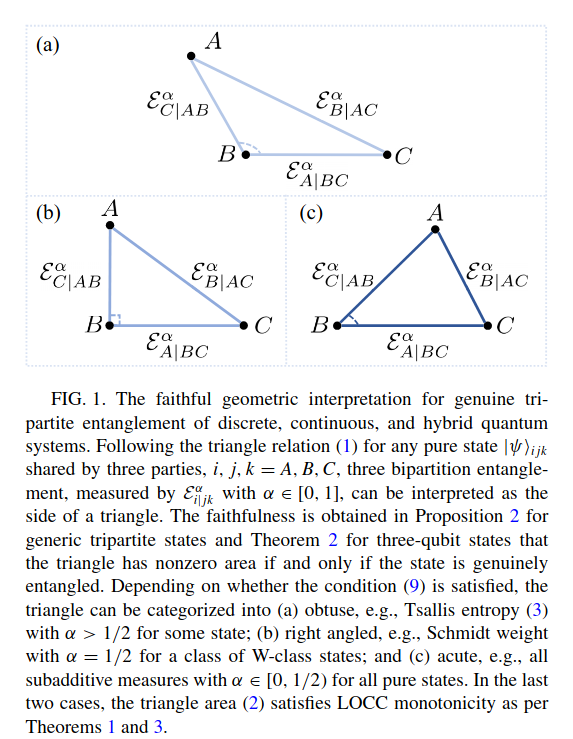
\includegraphics[width=0.5\linewidth]{figuras/ch2/triangulos.png}
    \caption{.}
    \label{fig2:triangulos}
\end{figure}
Lo que dicen es que dada una medida de entrelazamiento bipartito $\mathcal{E}^\alpha_{i|jk}$ definida sobre alguna partición del sistema total $ijk$, lo que se tiene es que
\begin{equation}
    A(\ket\psi_{ijk})=\sqrt{Q(Q-\mathcal{E}^\alpha_{i|jk})(Q-\mathcal{E}^\alpha_{j|ik})(Q-\mathcal{E}^\alpha_{k|ij})}
\end{equation}
con 
\begin{equation}
    Q=(\mathcal{E}^\alpha_{i|jk}+\mathcal{E}^\alpha_{j|ik}+\mathcal{E}^\alpha_{k|ij})/2
\end{equation}
para todo $\alpha\in(0,\frac{1}{2}]$, es una medida genuina de entrelazamiento. Para estados mixtos hacemos una suma usando el formalismo de convex-roof 
\begin{equation}
    A(\rho):= \inf_{\{p_m,\ket\psi_m\}}\sum_m p_m A(\psi_m)
\end{equation}
donde el mínimo es sobre todas las descomposiciones $\rho=\sum_mp_m\ket{\psi_m}\bra{\psi_m}$. Vamos a continuar en ingles para ir practicando escritura. This measure only captures 3-partite entanglement, but forgets about the cases where 2-partite entanglement is present. A trivial example is the case where we have a pure state $\ket{\psi_{EPR}}=\ket{0}\ket{\Phi_{BELL}}$, where $\ket{\Phi_{BELL}}$ is either of the four Bell states. In this trivial example, it is obvious that subsystems 2 and 3 are maximally entangled, but the area of the triangle is 0 because it is separable w.r.t subsystem 1. 

So the first thing to consider when ariving at this expresion is which entanglement measure to use for the bipartitions $\mathcal{E}^\alpha_{i|jk}$. My first two candidates are concurrence and VonNeumann Entropy, but both of them present different kinds of problems. Firstly, concurrence is well known and used for qubit-qubit systems, which is not the case for two of the bipartitions considered here. For concurrence to work, we should generelize it to higher dimensions and it should be able to "distinguish" between 2x2 and 2x3 systems, and have a kind of correspondance between both cases. Secondly, von Neumann entropy is a good measure, but only for pure states. As we have a pure state, perhaps it seems apropiate, but this is not correct because of the fact that the bipartitons of a pure state are not necesarily pure as well. In fact, if we have genuine 3-partite entanglement, it is expected that the reduced density matrices are mixed, and so the von Neuman entropy for the bipartitions is rendered unusable. A quick example shows that the pure state $\ket{GHZ}=(\ket{000}+\ket{111})/\sqrt{2}$ has a reduced density matrix $\rho_{ij}=\text{Tr}_k\ket{\psi}\bra{\psi}=\frac{1}{2}(\ket{00}\bra{00}+\ket{11}\bra{11})$ which is clearly mixed. It is well known that GHZ states are genuinly entangled. Moreover, as we showed, the reduced density matrix is mixed for any bipartition possible, this a hint of the 3-partiness of the entanglement for this particular state. There may be other states that only share entanglement between some parts of the system. A trivial example is en EPR pair of two qubits which we extend to have an aditional part $\ket{EPR}=(\ket{01}+\ket{10})/\sqrt{2}\otimes\ket{i}$. This state only has entanglement between the first two parts of the system. Therefor, not every bipartition of this state is mixed.

The consecuence of this is to look for either a generalized concurrence, for our purpose a qubit-qutrit concurrence will sufice, or to abandon this and use a better measure. As said before, because of the system we are using, and because we want to compute the entanglement for a unitary evolution, it is enough to have a qubit-qutrit entanglement measure, as in the diagonal blocks of the Tavis-Cummings evolution we can at most have a difference in 2 excitations in the cavity field mode. That is, we can think of the cavity as a 3 level system, or in a more inprecise manner, a qutrit. This is only possible if we consider unitary evolution and an initial condition with a well defined number of excitations in the system, so that the evolution reduces to a 3x3 space. It is worth noticing that for this triangle relation to work, the bipartite measure used should work for both $2\otimes2$ and $2\otimes3$ systems, as the bipartitions of the system are not all equal. In the paper that proposed the triangle relation, they examplify the triangle relation with different measures for bipartite entanglement, but most of them are not usefull for mixed states. I think this is wrong, or at least it could be better if we use a measure that can be used for mixed states. 

The triangle area is proved to be a genuine measure for tripartite entanglement insoforth $\mathcal{E}$ is a subadditive measure and $\alpha\in(0,\frac{1}{2}]$, because under this conditions it admits monotonoicity under LOCC.

Another maybe usefull relation for the triangle measure is the fact that they find upper and lower bounds for it:
\begin{equation}
    \min\frac{\sqrt{3}}{4}\{\mathcal{E}^{2\alpha}_{i|jk},\mathcal{E}^{2\alpha}_{j|ik},\mathcal{E}^{2\alpha}_{k|ij}\}\leq A(\ket{\psi}_{ijk})\leq \frac{\mathcal{E}^{2\alpha}_{i|jk}+\mathcal{E}^{2\alpha}_{j|ik}+\mathcal{E}^{2\alpha}_{k|ij}}{4\sqrt{3}}
\end{equation}

Now that, given a good bipartite measure, we have a genuine measure for tripartite entanglement, we must find a good bipartite measure for arbitrary dimension, i.e. a system composed of two qudits with a Hilbert space of dimension $D_1\otimes D_2$. It has to be usefull not only for one selected $D_1$ and $D_2$, but simultaneously for diferent dimensions. Particularly it will suffice that the measure works simultaneously for $2\otimes2$ and $2\otimes D$ dimensions, with $D\geq3$, and it must necesarilly work for mixed states, even if the global evolution remains unitary. 

My quest for a mixed state entanglement measure for a system of arbitrary dimensions starts with I-Concurrence \cite{}, a measure that generalices the concurrence by noting what the concurrence between two qubits represents, and applying this same reasoning to two arbitrary-dimensional systems. The measure comes from the notion that the concurrence is somewhat like the mean value of a inversion operator. As we know, the concurrence for two-qubit system is 

According to \cite{https://scispace.com/pdf/genuine-multipartite-entanglement-detection-and-lower-bound-1j5nw9cffj.pdf} the concurrence for a N-partite pure state $\ket{\psi}\in\mathcal{H}_1\otimes\mathcal{H}_2\otimes...\mathcal{H}_N\otimes$ is 
\begin{equation}
    C_N(\ket{\psi}\bra{\psi})=2^{1-\frac{N}{2}}\sqrt{(2^N-2)-\sum_\alpha \text{Tr}\{\rho_\alpha^2\}}
\end{equation}
If the state is mixed $\rho=\sum_ip_i\ket{\psi_i}\bra{\psi_i}$, then the concurrence is given by the convex roof 
\begin{equation}
    C_N(\rho)=\min_{\{p_i,\ket{\psi_i}\}}\sum_ip_iC_N(\ket{\psi_i}\bra{\psi_i})
\end{equation}
where the minimization is over all possible decompositions of $\rho$ in pure states. 
This makes sense, but why is the concurrence for a qubit-qubit system also well defined for mixed states? 

The concurrence for two bipartite systems can be given in terms of the eigenvalues of a matrix $R=\sqrt{\sqrt{\rho}\tilde\rho\sqrt{\rho}}$ with $\tilde\rho=(\sigma_y\otimes\sigma_y) \rho (\sigma_y\otimes\sigma_y)$. Then the concurrence is defined to be
\begin{equation}
    C(\rho)=\max\{0,\lambda_1-\sum_{i=2}^{\text{rank(R)}}\lambda_i\}
\end{equation}
where $\lambda_i$ are the eigenvalues of the matrix R in descending order $\lambda_1>\lambda_2>...$. 

To understand how to generalize concurrence we shall review how it is defined and it's propoerties following the work of Uhlmann \cite{http://arxiv.org/abs/quant-ph/9909060v4}. Given two vectors $\varphi$, $\psi \in \mathcal{H}\otimes\mathcal{H}^a$, where $\mathcal{H}^a$ is an ancilla, they reduce to 
\begin{align*}
    \rho&=\text{Tr}_a\ket{\varphi}\bra{\varphi} \\
    \omega & = \text{Tr}_a\ket{\psi}\bra{\psi}  
\end{align*}
First we define concurrence between $\rho$ and $\omega$ as
\begin{equation}
    C(\rho,\omega):= \max \{0,\lambda_1-\sum_{j>1}\lambda_j\}
\end{equation}

Then given a conjugation $\Theta$, an
 antiunitary satisfying $\Theta^2 = 1$. Writing $\Theta = \Theta^{-1} = \Theta^\dagger$ shows the hermiticity (self-adjointness) of conjugations. A conjugation $\Theta$ distinguishes in $\mathcal{H}$ a real subspace, $\mathcal{H}_\Theta$,
 consisting of all $\Theta$-invariant vectors, i.e. of all eigenvectors of $\Theta$ with eigenvalue 1. No real subspace in $\mathcal{H}$ is
 properly larger than $\mathcal{H}_\Theta$. Due to Hermiticity, $\Theta \psi = \psi$
 and $\Theta\phi = \phi$ result in
 $\langle\psi,\varphi\rangle=\langle\varphi,\psi\rangle$
 so that the scalar product becomes real if restricted to $\mathcal{H}_\Theta$. In other words, $\mathcal{H}_\Theta$ is not only a real subspace, it is a real Hilbert subspace. On the other hand, $\Theta$ can be gained as complex conjugation in every basis contained
 in $\mathcal{H}_\Theta$. This establishes a one–to–one correspondence between maximal real Hilbert subspaces and conjugations. So, given the conjugation $\Theta$ we define de $\Theta$-Concurrence as 
 \begin{equation}
     C_\Theta(\rho):=C(\rho,\tilde\rho), \; \; \tilde\rho=\Theta\rho\Theta
 \end{equation}
Afterwards they prove some properties and implications.

\textbf{Theorem 1}: Let $\Theta$ be a conjugation, then 
\begin{equation}
    C_\Theta(\rho)=\min\sum|\bra{\phi_k}\Theta\ket{\psi_k}|
\end{equation}
where the \textit{min} is taken over the ensemble $\{\phi_1,\phi_2,...\}$ such that
\begin{equation}
    \rho=\sum\ket{\phi_k}\ket{\psi_k}
\end{equation}
is valid. A direct consequence of the definition of concurrence is homogeneity, given a real numer $\mu$, $C_\Theta(\mu\rho)=\mu C_\Theta(\rho)$ $\forall \mu>0$.

Afterwards it is proven that $C_\Theta$ is \textit{convex}.

Next, we have to see how Optimal Decompositions work. Let $\Omega$ be the state space, if $\rho$ is in this space, a decomposition can be writen as 
\begin{equation}
    \rho=\sum p_k \pi_k, \;\; \pi_k=\frac{\ket{\phi_k}\bra{\phi_k}}{\braket{\phi_k}{\phi_k}}.
\end{equation}
If the decomposition is potimal, the $\Theta$-Concurrence can be writen as
\begin{equation}
    C_\Theta(\rho)=\sum p_kC_\Theta(\pi_k)
\end{equation}
Fixing a density operator $\rho$ and define an antilinear operator $\vartheta$ by
\begin{equation}
    \vartheta \equiv \vartheta_\Theta := \sqrt{\rho}\Theta\sqrt{\rho}.
\end{equation}
Because $\Theta^\dagger=\Theta$, $\vartheta$ is antilinearly Hermitian. The fact that $\Theta=\Theta^\dagger$ means that $\vartheta$ is antilinearly hermitian, then...

Now moving on to the \textbf{generalization of concurrence to more dimensions}, we follow some of the facts and measures used and derived in \cite{arXiv:2208.04745v1  [quant-ph]  2 Aug 2022}. In this work, the authors study the entanglement of certain $2\otimes3$ states, which are called TGX and SGX states. As this states are not of our interest, we will not dive into the details, however they use an entanglement measure that may be usefull for our porupose. Moreover, they give expresions for it and how to perform pure state decomposition. 

\subsubsection{Pure State Decomposition and Convex Roof Extension}\label{subsubsec:convex_roof_ext}

As said, we would like to extend an entanglement measure for pure states to mixed states. This procedure is well known \textit{Convex Roof Extension}, and consists of minimizing over all possible pure decompositions of the mixed state:
\begin{equation}
    E(\rho)=\inf_{\{p_j,\ket{\psi_j}\}}\sum_{j} p_j E(\ket{\psi_j}\bra{\psi_j}).
\end{equation}
To achive this, we have to take the minimum over all posible pure decompositions of the mixed state $\rho$. This could be a daunting task if the Hilbert space is big. The next question is then, how to find all pure decompositions of a given density matrix. A way to, do this is to take $\rho$ to its spectral decomposition. It is one of the posible pure decompositions:
\begin{equation}
    \rho=\sum\lambda_i\ket{\phi_i}\bra{\phi_i}
\end{equation}
where $\{\lambda_i,\ket{\phi_i}\}$ are the eigenvalues and corresponding eigenvectors of $\rho$. Then, we can take a unitary transformation defined by its matriz elements $U_{jk}$ and define a set of modified vectors
\begin{equation}
    \ket{\tilde w_j}=\sum_k U_{jk}\sqrt{\lambda_k}\ket{\phi_k}.
\end{equation}
Given this new vectors we can arrive at another expresion for the density matrix
\begin{equation}
    \rho=\sum_j p_j \ket{w_j}\bra{w_j},
\end{equation}
where $p_j=\braket{\tilde w_j}{\tilde w_j}$ and $\ket{w_j}=1/\sqrt{p_j}\ket{\tilde w_j}$. This means that we have a expresion that depends on the unitary transformation $U$:
\begin{equation}
    E(\rho)=\inf_{\{U\}} \sum p_j E(\ket{w_j}\bra{w_j}),
\end{equation}
where now the minimum is taken over all posible unitary transformations $U$. This means, our task is to minimize this function over all $U\in U(6)$, the unitary group $U(6)\in \mathbb{C}^{6\times6}$. The first thing to attempt is to parametrize this matrix group, but this turns out to be impossible, so the next step is to find a way to sample and take the minimum of this function over all possible $U$. This leads us to Random Matrix Theory (RMT), a usefull tool for this kinds of problems, where we have to evaluate a funtion over the manifold of unitary matrices. This is an interesting topic, but it will suffice to find some numerical way to randomly generate a matrix and some numerical way to span the manifold. For this, we found the python libraries \textit{pymanpot} \cite{JMLR:v17:16-177} and \textit{geomstats}, which in combination give us the numerical tools to explore the whole matrix manifold and optimize this function in a spart way, for example using gradiente descendiente and not only brute force. 

\section{Exploring optimization algorithms for entangled mixed states}

As in section \ref{subsubsec:convex_roof_ext}, we want to find the convex roof extension for the tripartite case. Therefor, we use Pymanopt and Autograd to solve this optimization problem in Python. 

To se which optimization algorithm implemented here works best, we will compute the entanglement of the 4x4 reduced density matrix of the two qubits tracing over the cavity $\rho_{AB}=\text{Tr}_C(\ket{\psi}\bra{\psi})$. As for a mixed two qubit state we can use the Conncurrence as a measure for entanglement, we will compare the Convex roof extension optimizatino for different measures and algorithms to see what combination is closer to the concurrence. With this analysis we will choose the best combination available to study tripartite entanglement. 
First using von Neuman entropy and Conjugate Gradient optimizer, we study if the parameter \textit{min\_step\_size} improves the algorithm. 


For now, the best algorithm seems to be the ParticleSwarm, using parameters max\_iterations=5 and population=25 seems reasonable, as it give good results and is not as computationally costly. Either way, the problem is that comparing the numerics, the convex roof extension is noisy in comparision to concurrence, and moreover it does not present entanglement sudden death. 

As this aproach seems to be numerically unstable and costly, we look for other alternatives. 

The next thing I found is Negativity. It seems to work for any bipartite system, independent of the dimensions, and doing some quick test, it also presents entanglement sudden death. As this seems to work, the next step is to try to make a tripartite entanglement measure using negativity, and doing an analysis of the dependence of the entanglement on the parameters of the problem. 

The main thing to look out for, is how we quantify the entanglement, since we have different kinds of entanglement in the system, that is, between any two parties, for example between A and B but tracing over C, then we have entanglement between A and B+C, and finally we have genuine tripartite entanglement. In total, 7 different kinds of entanglement. 
Another interesting question: Is it possible to find an entanglement invariant? Or some quantity that is invariant if the entanglement of the system remains constant? The goal of this is to see if during the evolution, the entanglement varies. Obviously, as it is easily available with numerics, the entanglement of the subsystems does change, but we do not have a precise defiintion of what entanglement means in this tripartite case. Maybe, if we have a general quantity that we now is entanglement invariant (whatever entanglement means in whatever dimension we are treating), it can tell us if the systems entanglement is actually changing or not.

\subsubsection{Negativity}\label{subsubsec:negativity}
La negatividad sirve para ver cuanto un estado esta de distancia a uno separable, usando la transposicion parcial. Esta caracteristica funciona porque las matrices densidades tienen que ser semidefinidas positivas, y la operacion transposicion parcial nos lleva de estados separables a estados separables, en este caso, siendo la matriz transpuesta parcialmente tambien una matriz (o observable) positivo. En cambio, si aplicamos la transposicion parcial sobre un estado entrelazado, entonces la matriz densidad resultante no es positiva, entonces si hacemos la suma de los autovalores negativos, tenemos una medida de cuanto el estado se aleja de ser separable. Formalmente, la negatividad se define como
\begin{equation}
    \mathcal{N}(\rho)=\sum_{\lambda<0}|\lambda|=\frac{||\rho^{T_A}||_1-1}{2}
\end{equation}
donde $||\cdot||_1$ es la norma 1, que es la suma de los valores absolutos de los autovalores, y $\rho^{T_A}$ es la transposicion parcial de $\rho$ sobre el sistema A. Esta medida es una buena medida de entrelazamiento, ya que es monotona bajo LOCC, y es computacionalmente simple. Cuando consideramos estados multipartitos, la negatividad no nos da una medida genuina de entrelazamiento entre las 3 partes, pero si nos da una idea de cuanto entrelazamiento hay entre dos partes del sistema. En este caso, hay 6 particiones o situaciones posibles. Las primeras tres constan en pensar el entrelazamiento que comparten A-(BC), es decir la negatividad de la matriz total $\rho_{ABC}$ traspuesta parcialmente sobre A, y lo mismo para B-(AC) y C-(AB). Estas tres particiones nos dan una idea de cuanto entrelazamiento hay entre una parte del sistema y las otras dos. Luego, tenemos las otras tres particiones, que son A-B (trazando sobre C), B-C (trazando sobre A) y A-C (trazando sobre B). Estas tres particiones nos dan una idea de cuanto entrelazamiento hay entre dos partes del sistema, considerando que la tercera no coopera en el sentido de LOCC, por lo tanto las otras dos partes pierden una parte del entrelazamiento (o no). 
Hay diferentes criterios de separabilidad y clasificaciones de entrelazamiento, que se pueden resumir con la siguiente tabla:
\begin{table}
    \centering
    \begin{tabular}{|c|c|c|c|c|}
    \hline
         & $E_A$ & $E_B$ & $E_C$ & $\tau_3$ \\
         \hline
         A-B-C & 0 & 0 & 0 & 0 \\
         \hline
         A-BC & 0 & >0 & >0 & 0\\
         \hline
         B-AC & >0 & 0 & >0 & 0\\
         \hline
         C-AB & >0 & >0 & 0 & 0\\
         \hline
         W & >0 & >0 & >0 & 0\\
         \hline
         GHZ & >0 & >0 & >0 & >0\\
    \hline
    \end{tabular}
    \caption{Clasificacion de entrelazamiento en sistemas tripartitos.}
    \label{tab:entrelazamiento_tripartito}
\end{table}
Realizando esto sobre nuestro sistema, obtenemos los siguientes resultados.
Primero veamos para condicion inicial $\frac{1}{\sqrt{2}}(\ket{eg1}+\ket{ge1})$, comenzando por lo mas similar a lo que teniamos antes, el entrelazamiento entre los dos atomos trazando sore la cavidad, esto lo llamamos $N_{01}$. Tambien tenemos la posibilidad de estudiar el entrelazamiento entre un atomo y la cavidad, trazando sobre el otro atomo, que llamamos $N_{02}$ y $N_{12}$. Esperamos que $N_{02}=N_{12}$ por la simetria del estado inicial. Finalmente tenemos la posibilidad de estudiar el entrelazamiento entre un atomo y el resto del sistema, que llamamos $N_0$ y $N_1$, y el entrelazamiento entre la cavidad y los dos atomos, que llamamos $N_2$.

En cada subplot variamos $\Delta$, y vemos que tambien vamos variando $\chi$ y $k-J$ segun vamos moviendonos para la izquierda o hacia abajo respectivamente. En estas simulaciones los valores de $\chi$ y $k-J$ son en cada direccion $a=0,g,2g$ para $a=\chi,k-J$. Tambien como comentario general para esta serie de graficos, notemos que la barra de colores esta normalizada diferente para cada grafico, esto se debe a que en algunos casos, no se alcanzan valores entre 0 y 1, y por lo tanto no se aprecian correctamente las oscilaciones, de esta manera, se contrasta mejor pero hhay que estar atentos a eso.
\begin{figure}
    \centering
    \includegraphics[width=0.8\linewidth]{figuras/ch2/negatividad/3x3 eg1+ $N_{01}$ 012 012.png}
    \caption{Negatividad $N_{01}$ para condicion inicial $\frac{1}{\sqrt{2}}(\ket{eg1}+\ket{ge1})$.}
    \label{fig2:N_01_eg1+}
\end{figure}
Vemos que estos graficos son muy similares a los que teniamos antes con la concurrence, donde encontramos estas regiones "interesantes". La diferencia principal es que la negatividad no va entre 0 y 1 como la concurrence, sino que va entre 0 y $1/2$. Aun asi es similar el comportamiento.  
\begin{figure}
    \centering
    \includegraphics[width=0.8\linewidth]{figuras/ch2/negatividad/3x3 eg1+ $N_{02}$ 012 012.png}
    \caption{Negatividad $N_{02}$ para condicion inicial $\frac{1}{\sqrt{2}}(\ket{eg1}+\ket{ge1})$.}
    \label{fig2:N_02_eg1+}
\end{figure}

\begin{figure}
    \centering
    \includegraphics[width=0.8\linewidth]{figuras/ch2/negatividad/3x3 eg1+ $N_{12}$ 012 012.png}
    \caption{Negatividad $N_{12}$ para condicion inicial $\frac{1}{\sqrt{2}}(\ket{eg1}+\ket{ge1})$.}
    \label{fig2:N_12_eg1+}
\end{figure}
Como es de esperar, los graficos de $N_{02}$ y $N_{12}$ son iguales, por la simetria del estado inicial. En estos casos, la negatividad parece casi contraria a la de $N_{01}$, en donde en uno vemos una zona muy oscura, donde hay muchoi entanglement sudden death, en el otro vemos oscilaciones de gran amplitud y no mucho sudden death. Esto lleva a pensar que el entrelazamiento se va pasando de uno al otro. Para comprobar esto deberiamos hacer un grafico mostrando la suma de los entrelazamientos a ver si se mantiene aproximadamente constante. La otra cosa a destacar es que las oscilaciones en estos dos graficos van entre 0 y 0.3, a diferencia del anterior donde oscilan entre 0 y 0.5. 

Ahora miremos las negatividades entre un subsistema con los otros dos, que son las cantidades $N_0$, $N_1$ y $N_2$. Estas representan, por ejemplo el $N_0$, el entrelazamiento entre el primer atomo y el resto del sistema, es decir el segundo atomo y la cavidad. Nuevamente esperamos que $N_0=N_1$ por la simetria del estado inicial. Esto parece efectivamente ser asi.
\begin{figure}
    \centering
    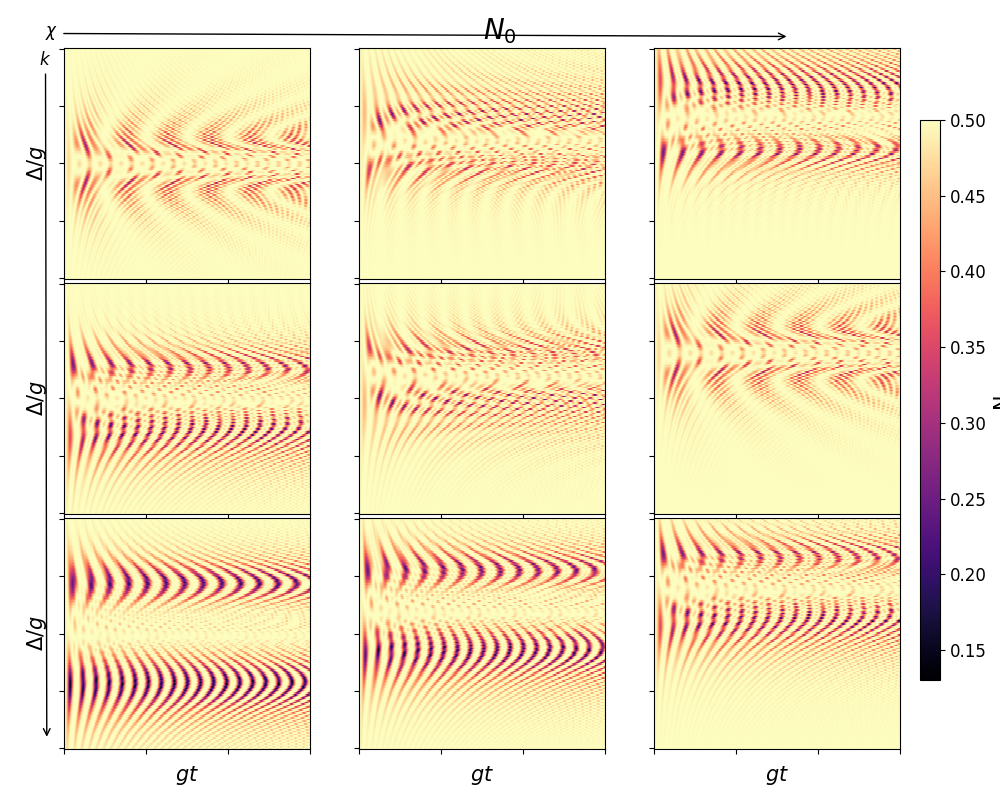
\includegraphics[width=0.8\linewidth]{figuras/ch2/negatividad/3x3 eg1+ $N_0$ 012 012.png}
    \caption{Negatividad $N_{0}$ para condicion inicial $\frac{1}{\sqrt{2}}(\ket{eg1}+\ket{ge1})$.}
    \label{fig2:N_0_eg1+}
\end{figure}

\begin{figure}
    \centering
    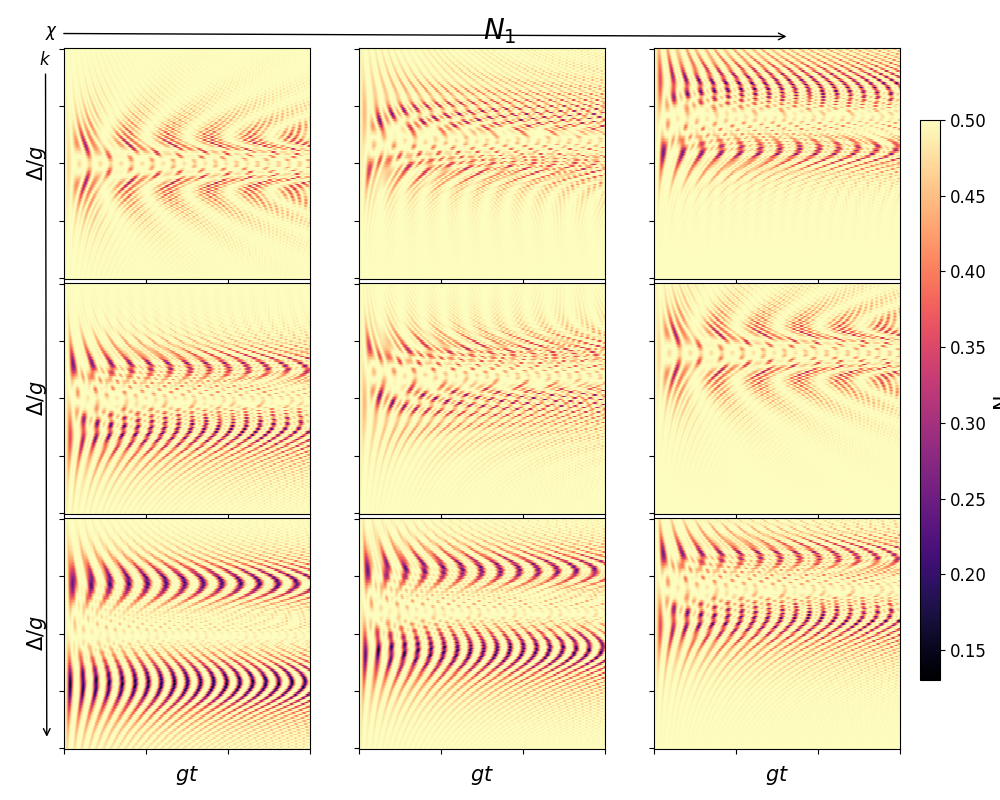
\includegraphics[width=0.8\linewidth]{figuras/ch2/negatividad/3x3 eg1+ $N_1$ 012 012.png}
    \caption{Negatividad $N_{1}$ para condicion inicial $\frac{1}{\sqrt{2}}(\ket{eg1}+\ket{ge1})$.}
    \label{fig2:N_1_eg1+}
\end{figure}
Mirando estos dos graficos, podemos observar como hay entrelazamiento bastante fuerte, y tambien vemos regiones oscilantes. Esto habria que analizarlo un poco mas en detalle pero esta interesante.
\begin{figure}
    \centering
    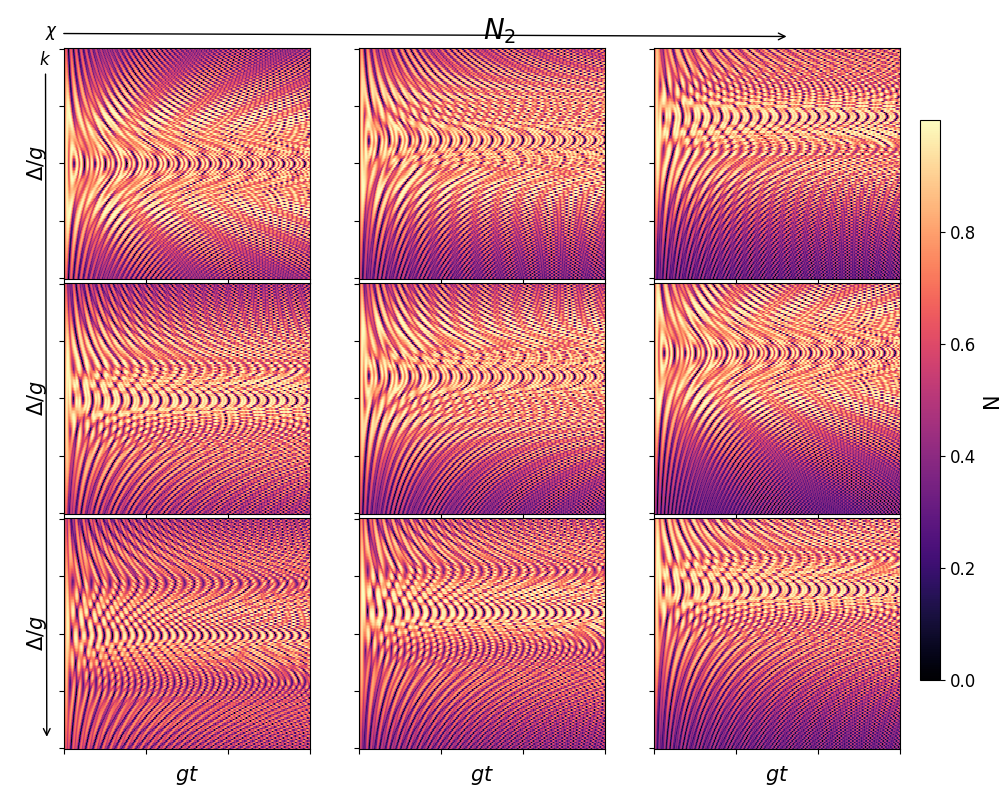
\includegraphics[width=0.8\linewidth]{figuras/ch2/negatividad/3x3 eg1+ $N_2$ 012 012.png}
    \caption{Negatividad $N_{2}$ para condicion inicial $\frac{1}{\sqrt{2}}(\ket{eg1}+\ket{ge1})$.}
    \label{fig2:N_2_eg1+}
\end{figure}
A diferencia del anterior, en este caso parece que mientras maor sea el detunning, menor es el entrelazamiento que comparte la cavidad con el resto del sistema, pero aun asi debemos diferenciar que en este grafico los colores estan normalizados entre practicamente 0 y 1, con lo cual quizas es un poco enganioso y hay que rehacer los graficos con la misma escala de colores para poder comparar un poco mejor.

Lo ultimo que tengo para decir es que, estaria bueno hacer un codiguito para estudiar lo que esta puesto en la tabla \ref{tab:entrelazamiento_tripartito}, donde nos fijamos tiempo a tiempo si las 3 negatividades son mayores a cero. Esto nos va a decir si hay entrelazamiento tripartito, o si solo hay entrelazamiento bipartito que se va moviendo entre las partes. Yo espero que haya algun entrelazamiento tripartito pero estaria bueno tener un grafico concreto que nos muestre con certeza. 

Las conclusiones son que podemos extender un poco mas el analisis del entrelazamiento que habiamos hecho antes. Todavia me queda estudiarlo a fondo, pero estaba mas concentrado en los otros proyectos y en leer otras cosas porque estaba un poco cansado y queria leer cosas nuevas. Pero ahora que hace algunas semanas que no lo toco mucho esto, me dieron ganas de analizar bien en profundidad esto y ver si podemos sacar una conclusion un poco mas fuerte. 

Tambien tenemos para otra condicion inicial. Los graficos van todos juntos en el apendice \ref{a}
\subsubsection{Schmidt Decomposition}
\text{https://arxiv.org/pdf/quant-ph/0610253} paginas 53-60 aprox

Se puede ver si queda invariante durante la evolucion. No deberia porque el entrelazamiento va cambiando, pero quizas es interesante ver como hace. Esta medida no es continua, ya que se basa en la descomposicion de schmidt y busca ver cual es el minimo posible de estados necesarios en la descomposicion. Entonces si es separable deberiamos tener $E_S=log_2(1)=0$, pero apenas sea un poquito entrelazado tenemos $E_S=log_2(2)=1$. Depende del tipo de entrelazamiento podesmo tener diferentes valores de $E_S$, pero son discontinuos.

\subsubsection{Ent: A Multipartite Entanglement Measure, and Parameterization of Entangled States}

Hoy encontre un paper que parece interesante. Lo tengo que leer a ver si me gusta y me convence. Escrito por  Samuel R. Hedemann  arXiv:1611.03882v3  [quant-ph]  18 Apr 2018.


